%  
%  in CH1 give an real life example at the begining as a BACKGROOUND
%  describe bacis concepts
%  and go into more details? obvious
%  
%  
%  
%  in CH2 active learning or web optimization
%  
%  
%  
\documentclass[12pt, a4paper, pdflatex]{report}
%  notitlepage - abstract on the same page
\usepackage{indentfirst} % indent frst paragraph of section
\usepackage{fullpage} % full A4 page
\usepackage{amsmath}
\usepackage[pdftex]{graphicx}
\usepackage{cite} % BiTeX
\usepackage{lipsum}
\newcommand{\ts}{\textsuperscript}
\usepackage[usenames,dvipsnames]{color}

% \usepackage{polski}
% \usepackage[polish,english]{babel}
% \usepackage[utf8]{inputenc}
\usepackage[T1]{fontenc} % polsih

% Code snippets
\usepackage{listings}
% \usepackage{color}

\definecolor{dkgreen}{rgb}{0,0.6,0}
\definecolor{gray}{rgb}{0.5,0.5,0.5}
\definecolor{mauve}{rgb}{0.58,0,0.82}

\lstset{frame=tb,
  language=R,
  aboveskip=3mm,
  belowskip=3mm,
  showstringspaces=false,
  columns=flexible,
  basicstyle={\small\ttfamily},
  numbers=none,
  numberstyle=\tiny\color{gray},
  keywordstyle=\color{blue},
  commentstyle=\color{dkgreen},
  stringstyle=\color{mauve},
  breaklines=true,
  breakatwhitespace=true
  tabsize=3
}
% END Code snippets

% $\backsim\ \sim\ \thicksim$

\newcommand{\HRule}{\rule{\linewidth}{0.5mm}}

\newenvironment{dedication}
  {\clearpage           % we want a new page
   \thispagestyle{empty}% no header and footer
   \vspace*{\stretch{1}}% some space at the top 
   \itshape             % the text is in italics
   % \raggedleft          % flush to the right margin
   \raggedright          % flush to the right margin
   \par\setlength{\leftskip}{0.3\textwidth}\noindent\ignorespaces
  }
  {\par % end the paragraph
   \vspace{\stretch{3}} % space at bottom is three times that at the top
   \clearpage           % finish off the page
  }

\begin{document}

\begin{titlepage}
\begin{center}
% Upper part of the page. The '~' is needed because \\
% only works if a paragraph has started.

\includegraphics[width=0.5\textwidth]{graphics/UOB-logo.png}~\\[4cm] % was 1cm

% \textsc{\LARGE University of Bristol}\\[1.5cm]

%\textsc{\Large Final year project}\\[0.5cm]

% Title
\HRule \\[0.4cm]
{ \huge \bfseries \emph{Multi-armed bandits} problem.\\
	Comprehensive introduction to the \colorbox{magenta}{problem} for everyone with real life application. \\[0.4cm] }
\HRule \\[1.5cm]

% Author and supervisor
\begin{minipage}{0.4\textwidth}
\begin{flushleft} \large
\emph{Author:}\\
Kacper B. \textsc{\textbf{Sokol}}
\end{flushleft}
\end{minipage}
\begin{minipage}{0.4\textwidth}
\begin{flushright} \large
\emph{Supervisor:} \\
Dr.~David \textsc{\textbf{Leslie}}
\end{flushright}
\end{minipage}

\vfill

% Bottom of the page
{\large \today}
\end{center}
\end{titlepage}

% \title{\emph{Multi-armed bandits} problem.\\
% 	Practical introduction to the problem for everyone.\\
% 	Real life application.}
% \author{Kacper Sokol\\University of Bristol, UK}
% \date{\today}
% \maketitle
% \begin{flushright}
% Supervised by:\\
% \textbf{David Leslie}
% \end{flushright}
% \begin{center}
% \line(1,0){250}
% \end{center}

\begin{abstract}
\thispagestyle{empty}% no header and footer
This dissertation consists of two chapters. First one is a comprehensive introduction to theory underlying multi-armed bandits problem. Reader is assumed not to need any prior knowledge in this field, only basics of statistics and probability theory are required. Second chapter is experimental part focused on ...
\begin{center}
Keywords: \textbf{multi-armed bandit, reinforcement learning, exploration vs. exploitation ...}
\end{center}
\end{abstract}

\begin{dedication}
I would like to thank my parents who support me both financially and mentally. For the guidance and advice they are providing so I can make right choices throughout life and fulfill my dream of studying abroad.\newline

It would also be a painful journey without my supervisor Dr.~David~Leslie who always served me with an advice how to ``read'' all the mathematical books not to get overwhelmed with heavy maths.\newline

Finally, big thanks to I.\ and J.\ who always take care of my leisure time even though it always lacks.\\[2cm]
% \foreignlanguage{polish}{}
\begin{flushright}
Dzi\k{e}kuj\k{e} mamo,\\
dzi\k{e}kuj\k{e} Tomek.
\end{flushright}
\end{dedication}


\newpage
\tableofcontents
% \newpage
\thispagestyle{empty}
\cleardoublepage
\pagestyle{plain}
\setcounter{page}{1}


\chapter{\texttt{\textbf{Exploration}} of multi-armed bandits theory.}
The \emph{multi-armed bandit} problem has been rapidly developing field of statistics and probability theory since early 20\ts{th} century. With a vastly growing number of \colorbox{magenta}{problems} that could be framed as a multi-armed bandit scenarios the field has become interest of many scientists, researchers, economists not to mention companies looking for work efficiency improvement and savings. All the solutions addressing these \colorbox{magenta}{problems} can be expressed as simple as finding a balance between \emph{exploration} and \emph{exploitation}.


\section{Background}
Many people know statistics and probability as analyzing processes or data in various aspects. They consider it as a rather \emph{static} science. But what if the process of our interest is continuously developing while we want to discover it or it demands our interaction. Simple statistics or probability might not be able to handle such cases as good as bandit theory.\\

To begin with, lets consider \emph{fruit machine} as it is a first thing that crosses reader's mind after hearing about multi-armed bandits. Imagine a row of slot machines in front of you. Pulling an arm of each of these automaton will result in different outcome (win or loose) each with corresponding probability according to some unknown distribution. Result for now on can be interpreted as various reels combinations. For the sake of simplicity it can be assumed that each automaton gives binary result: \emph{win} with probability $p$ and \emph{loose} with probability $p-1$. Without lost of any information row of such machines can be transformed into only one automation but with multiples arms or buttons each corresponding to single machine in a mentioned row.\\

The natural example that follows binary bandits is a row of coins, where some of them may be unfair. In presented scenario each coin corresponds to an \emph{Arm} of a bandit and tossing one of them for several times can be considered as realization of a Bernoulli process with unknown parameters.\\ If a player is rewarded when the outcome of a trial is \textbf{H}ead then the goal is to find the coin which has bias with maximum probability of \textbf{H} and play it forever.\\

If a gambler does not want to loose all possessed money really quick it would be probably a good idea to have some kind of strategy that maximizes chances of winning. It is assumed that the gambler is for the first time in a given casino so any prior information regarding expected return from each of the arm is assumed to be unknown. Initially random arm is chosen as all of them "look the same". On contrary, during the second turn selecting \emph{optimal} arm to play on becomes a serious dilemma that you might have not yet realized. The gambler faces a choice between already pulled arm with sample of expected return that is known and any other arm which for now on seem "the same" as there is no information about potential reward.\\
If gambler decides to take advantage of already known arm and pull it again we call this action \emph{exploitation}--- taking advantage of already checked possibilities. On the other hand, taking a risk and choosing one of unknown arms will result in gathering some more information about the system what is usually said to be \emph{exploration} step.


\section{Applications} % emphasized underlying
Multi-armed bandits is not just theory that one reads from a book and try to memorize, but it extends to many real life applications. This section is devoted to simple case study in which it seems natural to use "bandit approach". Applications are versatile ranging from drug testing and maximizing income from web advertisement through semi-supervised machine learning in modern computer science as well as time and budget management of research projects.\\

To begin with, imagine a clinic testing two new drugs for a certain disease. Patients are queuing up to receive a treatment. Assuming that doctor cannot refuse to treat anyone, for each person suffering from a disease (each \emph{Play}) there are two possible cures (two \emph{Arms}). The key assumption here is that the effect of chosen action occur immediately, in other words treated person either stays sick or the disease goes away (immediate \emph{Payoff}). The goal of a doctor is to maximize the number of cured people. This model defines two-armed bandit.\\

The second mentioned approach is nowadays widely incorporated by companies such as Google~\cite{AYPSze12}\cite{ASMB:ASMB874}, LinkedIn~\cite{Tang:2013:AAF:2505515.2514700}, Microsoft~\cite{graepel2010web}, Yahoo~\cite{Li:2010:CAP:1772690.1772758} to their services. Research groups of these companies are using bandits algorithms to choose best website layout and advertisements locations to increase "click-rate", improve recommendation systems or enhance performance of semi-supervised and active learning algorithms in a field of machine learning.\\

The bandit theory also plays a key role in experiment allocation with restricted time and budget~\cite{gittins+glazebrook+weber}. While considering research projects pending to be conducted with limited amount of resources such as scientist time and grant funding as \emph{Arms} of a bandit. The goal is to maximize the number of accomplished projects (\emph{Payoff}) before running out of money.\\

With all the above scenarios barely scratching the tip of the iceberg we are now focusing on foundations of multi-armed bandits theory that one needs to precisely describe the processes happening "behind the scene".

\section{Structure of this chapter}
We begin with introducing the reader with necessary notation and nomenclature. Then we are moving to basic process description. Next proved optimal solutions of multi-armed bandits problem are described. Finally we form conclusions and highlight ongoing research with possible results and influence on applications.


\section{Terminology}
More scientific definition of "simple" multi-armed bandit in a statistical decision theory defines it as: sequential selection from $N \geq 2$ stochastic processes--- generally called \emph{Arms}, where both time and processes may be discrete or continuous. The goal is typically to recover unknown parameters which characterize stochastic processes behind each of the \emph{Arm} to maximize expected \emph{Payoff}.

It is very useful to be familiar with most common terms used to describe multi-armed bandit in papers and books. The basic concepts are listed below.
\begin{description}
\item[Multi-armed bandit ($N$)]--- a ``device'' with $N \geq 2$ possible choices of action (\emph{Arms}).
\item[Strategy ($\tau$)]--- tells the \emph{Agent} which \emph{Arm} to pull at given stage of \emph{Game}. A strategy is \emph{optimal} if it yields maximal expected \emph{Payoff}.
\item[Arm]--- one of $N$ actions that may be taken by \emph{Agent}. An \emph{Arm} is \emph{optimal} if it the best selection when following some \emph{optimal} strategy.
\item[Play]--- an \emph{Arm} pulled at stage $m$ of the \emph{Game} (i.e.\ one turn).
\item[Agent]--- a person that decides which \emph{Arm} to pull based on \emph{Strategy} $\tau$.
\item[Game]--- a sequence of \emph{Arms} pulled based on chosen \emph{Strategy} $\tau$.
\item[Payoff]--- a return of a game such as \emph{win--loose} or \emph{amount} of money gained.
\item[Discount series]--- factors that define how valuable is each of \emph{Payoffs}. For example only first $m$ outcomes may count and all the rest is neglected or the longer the \emph{Game} is ran the less particular outcome counts toward overall expected \emph{Payoff}.
\end{description}


\section{General assumptions}
Two fundamental assumptions to vast majority of bandit problems regard benefits from selecting an arm, namely:
\begin{itemize}
\item immediate \emph{Payoff} i.e.\ \emph{Agent} knows result of taken action straight away,
\item information gathered after a \emph{Play} can be used to modify chosen \emph{Strategy}.
\end{itemize}
Moreover in some cases we may restrict the memory of an \emph{Agent} to last $s$ outcomes. Therefore, selected \emph{Strategy} $\tau$ can relay on up to $s$ previous \emph{Plays}. These bandits approaches are called \emph{finite memory}.\\
Majority of this dissertation assumes that \emph{Arms} are independent. If this setting changes it will be clearly stated.


\section{Discount Sequence}
To specify the rules governing the ``significance'' of outcome from a single play at stage $m$ the \emph{discount sequence} is introduced. It is a vector $\mathbf{A}$ of specified length, which can also be infinite.
$$
\mathbf{A} = \left( \alpha_1, \alpha_2, \alpha_3, ... \right)
$$
When an \emph{Arm} is selected the discount sequence is modified as follows:
$$
\left( \alpha_1, \alpha_2, \alpha_3, ... \right)
\rightarrow
\left( \alpha_2, \alpha_3, \alpha_4, ... \right)
$$

\subsection{Observable and non-observable sequences}
\lipsum[1]


\subsection{Most common sequences}
There are many different discount sequences used with multi-armed bandits each with numerous assumptions. In the literature only two of them are described in great detail and both are presented below.
{
\subsubsection{Uniform sequence}
This discount sequence is most commonly used when a player wants to maximize the payoff of first $h$ outcomes.
The $h$-horizon uniform discount sequence is defined as:
\[
 \alpha_i =
  \begin{cases}
   1 & \text{for } i \leq n \\
   0 & \text{for } i > n
  \end{cases}
\]
leading to:
\[
  \mathbf{A} = ( \underbrace{ 1, 1, 1, ..., 1}_{h\text{ elements}}, 0, 0, 0, ... ) \text{ .}
\]\\
\\
Here after \emph{Arm} selection the horizon of discount sequence is decreased by $1$.


\subsubsection{Geometric sequence}
The geometric discount sequence is expressed with components $\alpha_i = a^{i-1}$ for some $a \in ( 0, 1 )$ resulting in:
$$
\mathbf{A} = \left( a^0, a^1, a^2, ... \right)
$$
where $\alpha_1 = a^0$ is always equal to $1$.\\
\\
On the other hand, here after \emph{Arm} selection the discount sequence is proportional to original sequence.\\
\\

}
In case of both sequences the decision problem and optimal strategy is unchanged if a discount series is multiplied by some constant. Furthermore, in case of geometric sequence is effectively the same the same throughout the \emph{Game}.

\subsection{Random discounting}
\subsection{Infinite horizon }

\subsection{Non-monotone sequences}



\section{Bandits settings}
\subsection{Real time, random bandits}
\subsection{Information gathering}
\subsection{Dependant \emph{Arms}}



\section{Seeking optimal solution}
In this section I will present number of approaches to find and optimal solution.\\
Blah blah blah blah.
Strategy id balancing exploration and exploitation to find optimal solution. Sometime it demand sanctifying early payoff to gain some more information about the system and maximize future payoff.
Information vs.\ immediate payoff. -- in hospital example case it means that sacrificing good of early coming patients by means of experimenting means improvement over time and better results of treatment on future patients.
To democratize it we can use geometric sequence so health of current patients is the same in comparison to future patients.\\
\\
\\
\\
This result shows that when the discounting is geometric, a bandit problem involving k independent arms can be solved by solving k different two-armed bandits, each involving one known and one unknown arm.\\

\subsection{Index approach (Gittins Index)}



\subsection{Bayesian approach}
Bayes' theorem allows for "straight forward" application to adaptive learning so it's a good approach tool in sequential decision making 

\subsection{Strategy comparison}

\subsection{Minimax approach}

\subsection{Finite memory strategy}
\subsubsection{'Stay on a winner'}

\subsection{Myopic strategies}
Not good in general.

\subsection{Thompson Sampling approach}
As all the rest of methods is well described in literature and they were main subject of interest it is relatively easy to find good texts about them. On contrary, Thompson Sampling is cutting edge approach with a lot of research going on the focus will be put on it and it will be described in deep details in  \textbf{Section~\ref{sec:thompsonsampling}} which is devoted to Thompson Sampling approach to finding an optimal strategy.

\subsection{etc.\ based on Google paper}



\section{Thompson Sampling\label{sec:thompsonsampling}}
To fully develop \emph{Thompson Sampling} approach to multi-armed bandit theory, two concepts need to be introduced:
\begin{itemize}
\item Bayesian statistics \emph{and}
\item sampling theory.
\end{itemize}
It is possible to use any probability distribution with \emph{Thompson Sampling} but for the sake of simplicity we will focus in this paper only on \emph{normally} distributed data. This restriction does not mean that it is not possible to apply this technique with any other distribution but due to space constrains the theory will be presented with \emph{normal likelihood}. Furthermore, discussing other scenarios of Thompson Sampling would demand from reader to be familiar with analytic approach to Bayesian \emph{posteriors}, \emph{priors} and \emph{likelihoods}.

\subsection{Bayesian statistics}
In this section we will shortly introduce normal distribution. Then we will discuss its aspects with regard to Bayesian statistics.

\subsubsection{The normal distribution}
The most common distribution in statistics with well known bell-shaped (see \emph{Figure~\ref{fig:normaldist}}) plot is the normal distribution also called \emph{Gaussian} distribution. If a random variable $\mathrm{X}$ follow such distribution parametrized by \emph{mean} $\mu$ and \emph{standard deviation} $\sigma$ we commonly write $\mathrm{X} \sim \mathcal{N}\left( \mu, \sigma^2 \right)$. Probability density function of $\mathrm{X})$ is:
$$
f \left(x | \mu, \sigma \right) = \frac{1}{\sigma \sqrt{2 \pi }} e^{- \frac{ {\left (  x - \mu \right )}^2 }{2 \sigma^2} }
$$
where the first part ${\left( \sigma \sqrt{2 \pi } \right)}^{-1}$ is a normalizing factor and the later part is a distribution ``kernel''.
$$
\int_{-\infty}^{+\infty} \! f \left(x | \mu, \sigma \right) \, \mathrm{d}x = 1
$$
with area under curve from $-\infty$ to $+\infty$ integrating to $1$~\cite{rice1995mathematical}.


\begin{figure}[htbp]
\centering
\includegraphics[width=0.5\textwidth]{graphics/normalpdf.pdf}
\begin{tiny}
\caption{Probability density function of normal distribution $\mathcal{N}\left( 0, 5 \right)$ in characteristic bell shape created in \texttt{R} (Snippet in \emph{Appendix~\ref{snip:normaldist}}).\label{fig:normaldist}}
\end{tiny}
\vspace{1cm}
\end{figure}



\subsubsection{\emph{prior}, \emph{posterior} and \emph{likelihood} distributions}
The next concept that we introduce is the dependency between prior, posterior and likelihood of a particular distribution. To illustrate it the \emph{normal} distribution will be used for the reasons mentioned above. The generalization to other distributions is straight forward~\cite{gelman2003bayesian}.\\

The basic theorem underlying all this section is called Bayes' theorem for point probabilities and states:
$$
p \left( \mathrm{B} | \mathrm{A} \right) = \frac{  p \left( \mathrm{A} | \mathrm{B} \right) p \left( \mathrm{B} \right) }{ p \left( \mathrm{A} \right) }
$$
\begin{center}
or
\end{center}
$$
p \left( \mathrm{B} | \mathrm{A} \right) \propto p \left( \mathrm{A} | \mathrm{B} \right) p \left( \mathrm{B} \right)
$$
where:
\begin{description}
\item[$p \left( \mathrm{B} | \mathrm{A} \right)$] is \textbf{posterior}--- being conditional probability of event \textrm{B} given event \textrm{A},
\item[$p \left( \mathrm{A} | \mathrm{B} \right)$] is \textbf{sampling density (``likelihood'')}--- being conditional probability of event \textrm{A} given event \textrm{B},
\item[$p \left( \mathrm{B} \right)$] is \textbf{prior}--- being marginal probability of event \textrm{B} and
\item[$p \left( \mathrm{A} \right)$] is \textbf{marginal} probability of event \textrm{A} (data) being normalizing factor.
\end{description}

Now we will focus on general results of Bayesian statistics when our likelihood function is normally distributed. From this point onwards we can develop a couple of different scenarios described below.\\

\textbf{\textrm{Non-informative prior. }}If we are lacking information about prior distribution the best that can be done is to minimize its influence on the inference. According to \emph{principle of insufficient reason} proposed by Bayes and Laplace we should assume that prior is \emph{uniformly} distributed so all outcomes are equally likely. We also assume that it is distributed over the real line for both $\mu$ and $\log \sigma^2$ (transformation to $\log$ scale is performed because $\sigma^2$ is non-negative quantity and it results in stretch along real line). These operations result in joint probability $p \left( \mu, \sigma^2 \right) \propto \frac{1}{\sigma^2} $ leading to posterior distributions given by $p \left( \mu | \mathrm{X}, \sigma^2 \right) \sim \mathcal{N} \left( \bar{x}, \frac{\sigma^2}{n} \right) $ and $p \left( \sigma^2 | \mathrm{X}, \mu \right) \sim \mathrm{Inv}\text{-}\mathrm{Gamma} \left( \frac{n}{2} , \sum_{i} \frac{\left( x_i - \mu \right)^2}{2}  \right) $ (inverse gamma distribution). This approach is not perfect and its criticism is widely known but for our application it suffices~\cite{Syversveen98noninformativebayesian}.\\

% give equation for normal likelihood --- uniform prior

\textbf{\textrm{Informative prior. }}It is the opposite scenario to one described above. With known distribution of the prior the application of Bayesian statistics is straight forward. From this point onward we will assume that our prior is informative with normal distribution.\\

\textbf{\textrm{Known variance. }}Firstly we will consider \emph{normal prior--normal likelihood} with $\sigma^2$ known and $\mu$ unknown (our variable).
$$
f \left( \mu | \mathrm{X} \right) \propto f \left( \mathrm{X} | \mu \right) f \left( \mu \right)
$$
The $\sigma^2$ in the notation is omitted for clarity purposes. In this case out prior is defined as follows:
$$
f \left( \mu \right)    \sim   \mathcal{N}\left( \mu, \tau^2 \right)
%                        ~
$$
giving:
$$
f \left( \mu \right)    =     \frac{1}{\sqrt{2\pi} \tau} e^{- \frac{{\left( \mu - M \right)}^2}{2 \tau^2} }
$$
where $M$ is prior mean and $\tau^2$ is variance of $\mu$ round $M$; likelihood is given by:
$$
f \left( \mathrm{X} | \mu \right)     \sim    \mathcal{N}\left( \mu, \sigma^2 \right)
$$
resulting in:
$$
f \left( \mathrm{X} | \mu \right)    =     \prod_{i=1}^{n} \frac{1}{\sqrt{2\pi} \sigma} e^{- \frac{{\left( \mu - x_i \right)}^2}{2 \sigma^2} }
$$
where $x_i \in X$ are data points.\\
After plugging both of them into Bayes rule we get:
$$
f \left( \mu | \mathrm{X} \right)     \propto     \frac{1}{\sigma \tau} e^{ -\frac{ {\left( \mu - M \right)}^2 }{2 \tau^2} -\frac{ \sum_{i=1}^{n} {\left( \mu - x_i \right)}^2 }{2 \sigma^2} }
$$
what clearly contains a kernel of normal distribution. After some algebraic transformation we finally get that posterior is \textbf{normally} distributed with mean $\epsilon$ and variance $\delta^2$ ( $f \left( \mu | \mathrm{X} \right) \sim \mathcal{N} \left( \epsilon, \delta^2 \right) $ ):
\begin{eqnarray*}
\epsilon &=& \frac{\sigma^2 M + n \tau^2 \bar{x}}{n \tau^2 + \sigma^2} = \frac{ \frac{1}{\tau^2} }{ \frac{1}{\tau^2} + \frac{n}{\sigma^2} }M + \frac{ \frac{n}{\sigma^2} }{ \frac{1}{\tau^2} + \frac{n}{\sigma^2} } \bar{x} \\
\delta^2 &=& \frac{\sigma^2 \tau^2}{n \tau^2 + \sigma^2} = \frac{ \frac{\sigma^2}{n} \tau^2 }{ \tau^2 + \frac{\sigma^2}{n} } \text{ .}
\end{eqnarray*}
\\

\textbf{\textrm{Unknown variance. }}This is more realistic case when the posterior is:
$$
p \left(  \mu, \sigma^2 | \mathrm{X} \right) \propto p \left( \mathrm{X} | \mu, \sigma^2 \right)    p \left( \mu, \sigma^2 \right) \text{ .}
$$
We now need to specify the details of prior distribution. One way is to assume independent distributions of both $\mu$ and $\sigma^2$ and establish separate priors for each.\\



In both later cases the posterior is normally distributed.\\
Basic results that yields from Bayesian statistics for normal distribution are available in wide variety of books so only useful results are presented. For more details regarding normal and other distributions please refer to~\cite{gelman2003bayesian}\cite{lynch2007introduction}.\\

\subsection{Sampling}
In general sampling is a technique used in statistics to select at random a subset of individuals or data points from a population of interest. To goal of such procedure is to gather representative group which holds the properties of original population. The main advantage of such approach is lowering the amount of data to process.\\
In our approach we use sampling to draw at random from particular pool (\emph{arm}) with unknown distribution.

\subsection{Introduction to Thompson Sampling}
start writing about Thompson sampling

\begin{figure}[htbp]
\centering
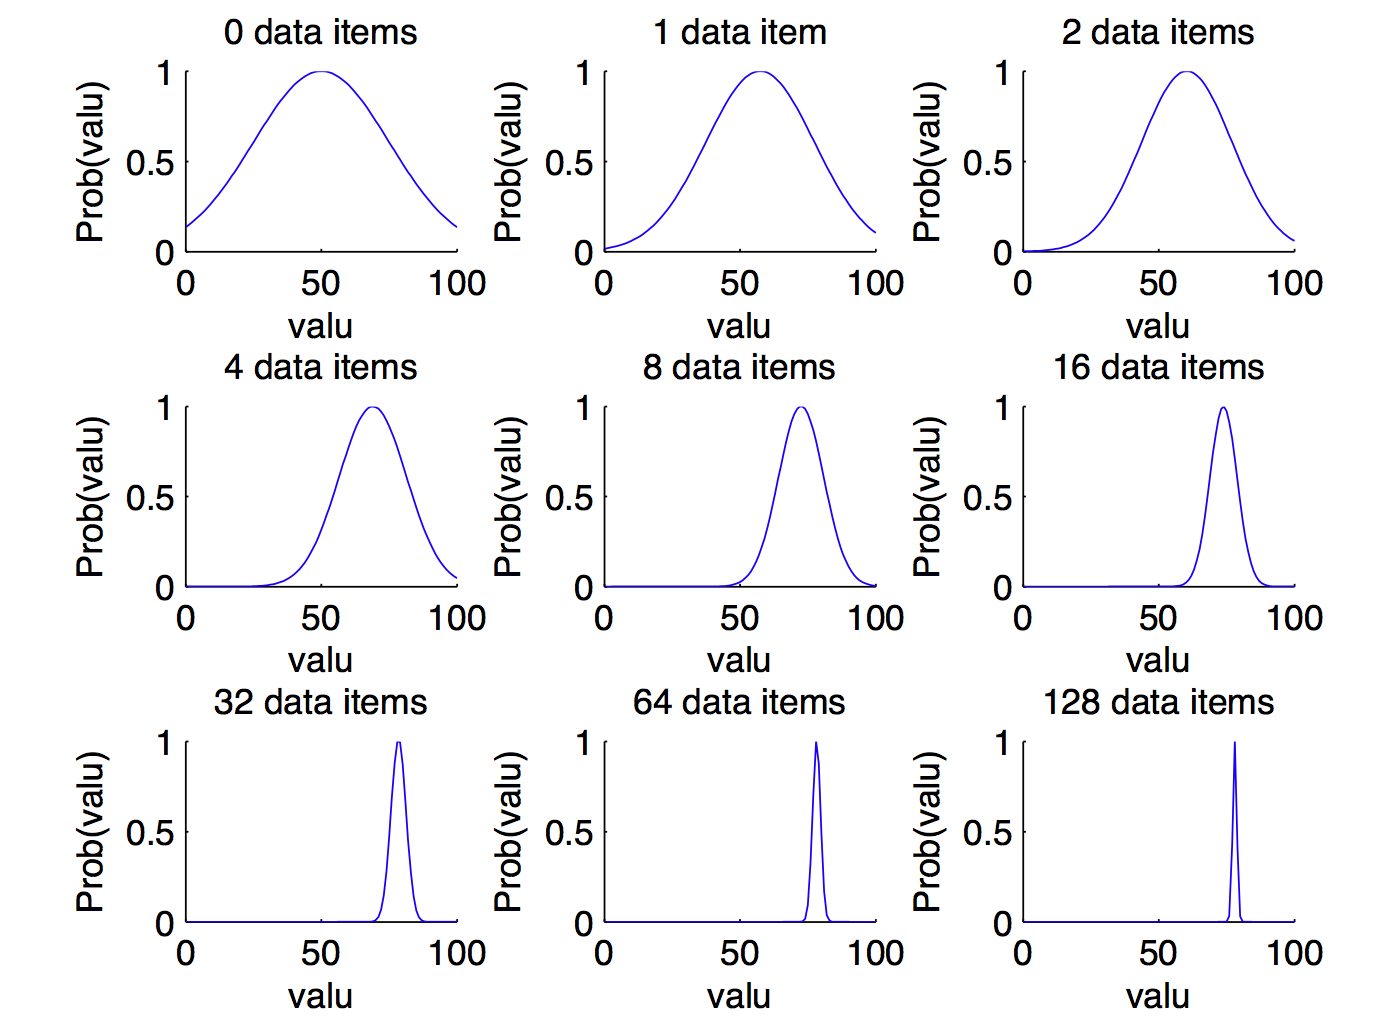
\includegraphics[width=0.7\textwidth]{graphics/sampling.png}
\begin{tiny}
\caption{Sampling and updating posterior probability density function of normal distribution $\mathcal{N}\left( \mu , \sigma^2 \right)$ (Figure taken from~\cite{Jacobs2008normalnormal}).\label{fig:sampling}}
\end{tiny}
\vspace{1cm}
\end{figure}








\chapter{Practical application--- \texttt{\textbf{Exploitation}} of multi-armed bandits optimal solution algorithms.}

\appendix
\chapter{Code snippets}

\label{snip:normaldist}PDF of normal distribution with mean $0$ and standard deviation $5$.
\begin{lstlisting}
x   <- seq(-30,30,length=10000)
y   <- dnorm(x,mean=0, sd=5)
plot(x,y, type="l", lwd=1)
\end{lstlisting}

\label{snip:thompsonsampling}Creating multiple normal distributions to visualize Thompson sampling.
\begin{lstlisting}
 x   <- seq(5,15,length=1000)
 y   <- dnorm(x,mean=10, sd=30)
plot(x,y, type="l", lwd=1)
sam <- sample(x, 10)
points(sam,dnorm(sam, 10, 1), col="green")

# for a few distributions
\end{lstlisting}


\newpage
\begin{center} \textbf{\huge \vspace*{15pt} FIN~\cite{berry+firstedt}} \end{center}

\bibliography{ref}{}
\bibliographystyle{plain}

\end{document}
